%versi 2 (8-10-2016)
\chapter{Analisis}
\label{chap:analisis}

Bab ini akan menjelaskan mengenai analisis sistem merujuk pada hasil studi yang telah dibahas pada bab sebelumnya. Pada bab ini juga akan dibahas perancangan sistem secara umum yang ditunjukkan dalam bentuk \textit{flowchart} dan \textit{usecase diagram}

\section{Deskripsi Sistem}
\label{sec:skripsi} 
%   Perangkat lunak yang dibangun tidak dibatasi oleh jenis arsitektur WSN yang dapat dipilih. Jenis arsitektur WSN \textit{flat} ataupun \textit{hirakikal}, dapat digunakan dalam perangkat lunak yang dibangun. Jenis komunikasi \textit{single-hop} ataupun \textit{multi-hop} dapat digunakan pada arsitektur hirakikal seperti yang dibahas pada subbab \ref{Arsitektur WSN}. 
  
   Perangkat lunak yang dibangun merupakan aplikasi yang berfungsi untuk memantau kondisi tanah sawah. Pemantauan dilakukan dengan menggunakan sensor-sensor yang terhubung dalam jaringan yang berfungsi untuk melakukan pengambilan variabel-variabel yang mempengaruhi kualitas tanah sawah. Variabel tanah yang mempengaruhi kualitas tanah sawah antara lain, kadar keasaman tanah (pH tanah), tingkat kelembaban tanah, suhu tanah, suhu dan kelembaban udara persawahan. Pengambilan data dari variabel-variabel tersebut akan dilakukan oleh sensor secara \textit{real-time}, dan ditampilkan ke komputer pengguna. Pengguna dari perangkat lunak yang dibangun dapat mengetahui kualitas tanah sawah yang dikelolanya, berdasarkan data yang dihasilkan dari kegiatan pemantauan. Dari data yang dihasilkan oleh perangkat lunak, pengguna diharapkan dapat terbantu dalam menentukan jenis perawatan terhadap tanah sawah yang dikelola.
   
   
   Secara sederhana proses yang dilakukan dalam pembangunan aplikasi ini adalah sebagai berikut. Sensor-sensor node disebar di area persawahan dan melakukan \textit{sensing} terhadap tanah yang diteliti. Sensor-sensor tersebut akan saling berkomunikasi untuk mengirimkan hasil \textit{sensing} yang didapatkannya ke \textit{base station}. \textit{Base station} akan menerima semua hasil \textit{sensing} sensor yang disebar untuk diteruskan dan ditampilkan ke layar komputer.
  
 
  
%\dtext{11-12} 

\section{Analisis Arsitektur dan Topologi WSN}
\label{sec:latex}

    
    Sensor node yang digunakan pada penelitian ini adalah sensor Arduino Mega 2560. Seperti yang dijelaskan pada subbab \ref{Pemrograman Arduino}, Arduino Mega merupakan pengembangan dari Arduino Uno yang merupakan jenis mikrokontroler paling populer. Jumlah pin yang lebih banyak pada Arduino Mega, memungkinkan lebih banyaknya node \textit{sensing} yang dapat di\textit{attach} pada papan untuk mengambil data tanah persawahan. Selain itu Arduino Mega juga dapat menyimpan data (bersifat sementara) hasil \textit{sensing} lebih banyak dibandingkan Arduino Uno.
    
    
    Sensor \textit{sensing} yang akan digunakan dalam penelitian ini antara lain, sensor pengukur pH tanah (ETP306), sensor kelembaban (FC28), sensor suhu tanah (DS18B20), sensor suhu udara(DHT11), dan \textit{Wireless Data Transceiver}(NRF24L01). Sensor ETP306 digunakan untuk mengambil data kadar keasaman dari tanah sawah yang diteliti. Sensor FC28 \textit{attach} dengan seri sensor MH untuk dapat terhubung dengan node sensor. Sensor FC28 digunakan untuk melakukan \textit{sensing} kadar kelembaban tanah. Untuk mengetahui suhu tanah, sensor DS18B20 akan dihubungkan dengan node sensor. Sensor FC28 dan DS18B20 harus secara langsung ditancapkan kedalam tanah sawah yang diteliti, untuk mengambil data dan melakukan \textit{sensing}. Sensor DHT11 dapat langsung \textit{attach} pada pin yang berada pada node sensor dan memberikan informasi suhu dan kelembaban udara sekitar persawahan. \textit{Wireless Data Transceiver} (NRF24L01) merupakan modul komunikasi \textit{wireless} yang dapat digunakan pada perangkat keras Arduino ataupun Raspberry. Seluruh sensor sensing tersebut akan terhubung dalam satu buah node sensor. Untuk \textit{base station} jenis perangkat keras yang akan digunakan adalah Raspberry pi 2 B+ yang memungkinkan pemrograman dilakukan pada sistem operasi Windows, seperti yang dibahas pada subbab \ref{Jenis Raspberry}.
    
     Perangkat lunak yang dibangun memfokuskan dalam melakukan \textit{sensing} terhadap tanah sawah yang diteliti dan melakukan komunikasi, agar data yang dihasilkan dapat dikirimkan sampai di \textit{base station}, untuk diteruskan ke komputer atau pengguna. Berdasarkan pembahasan pada subbab \ref{Arsitektur WSN} mengenai arsitektur WSN, pemilihan jenis arsitektur WSN \textit{flat} akan lebih baik untuk diimplementasikan. Arsitektur WSN flat tersebut dipilih berdasarkan luasnya wilayah penelitian yang tidak terlalu besar, dan jenis \textit{task} dari setiap node yang disebar yang memiliki tugas yang sama (melakukan \textit{sensing}).
     
     
    Topologi yang akan diuji pada perangkat lunak yang dibangun adalah topologi \textit{star}, topologi \textit{linear}, dan topologi \textit{partially connected mesh}, seperti yang telah dibahas pada subbab \ref{Topologi WSN}. Topologi \textit{linear} dipilih sebagai dasar dari topologi lainnya dan menjadi basis komunikasi antar node. Pada topologi \textit{star}, \textit{central node} akan berperan sebagai \textit{base station} (bersifat aktif) yang merupakan Raspberry pada perangkat lunak yang dibangun. Sedangkan node-node lainnya akan bertugas untuk melakukan \textit{sensing}. Topologi \textit{partially connected mesh} dibangun sebagai penguji diantara jenis topologi jaringan lainnya dan memungkinkan minimalnya gangguan yang terjadi pada topologi lainya, seperti yang dijelaskan pada subbab \ref{Topologi WSN}.

    \begin{figure}[H]
    	\centering  
    	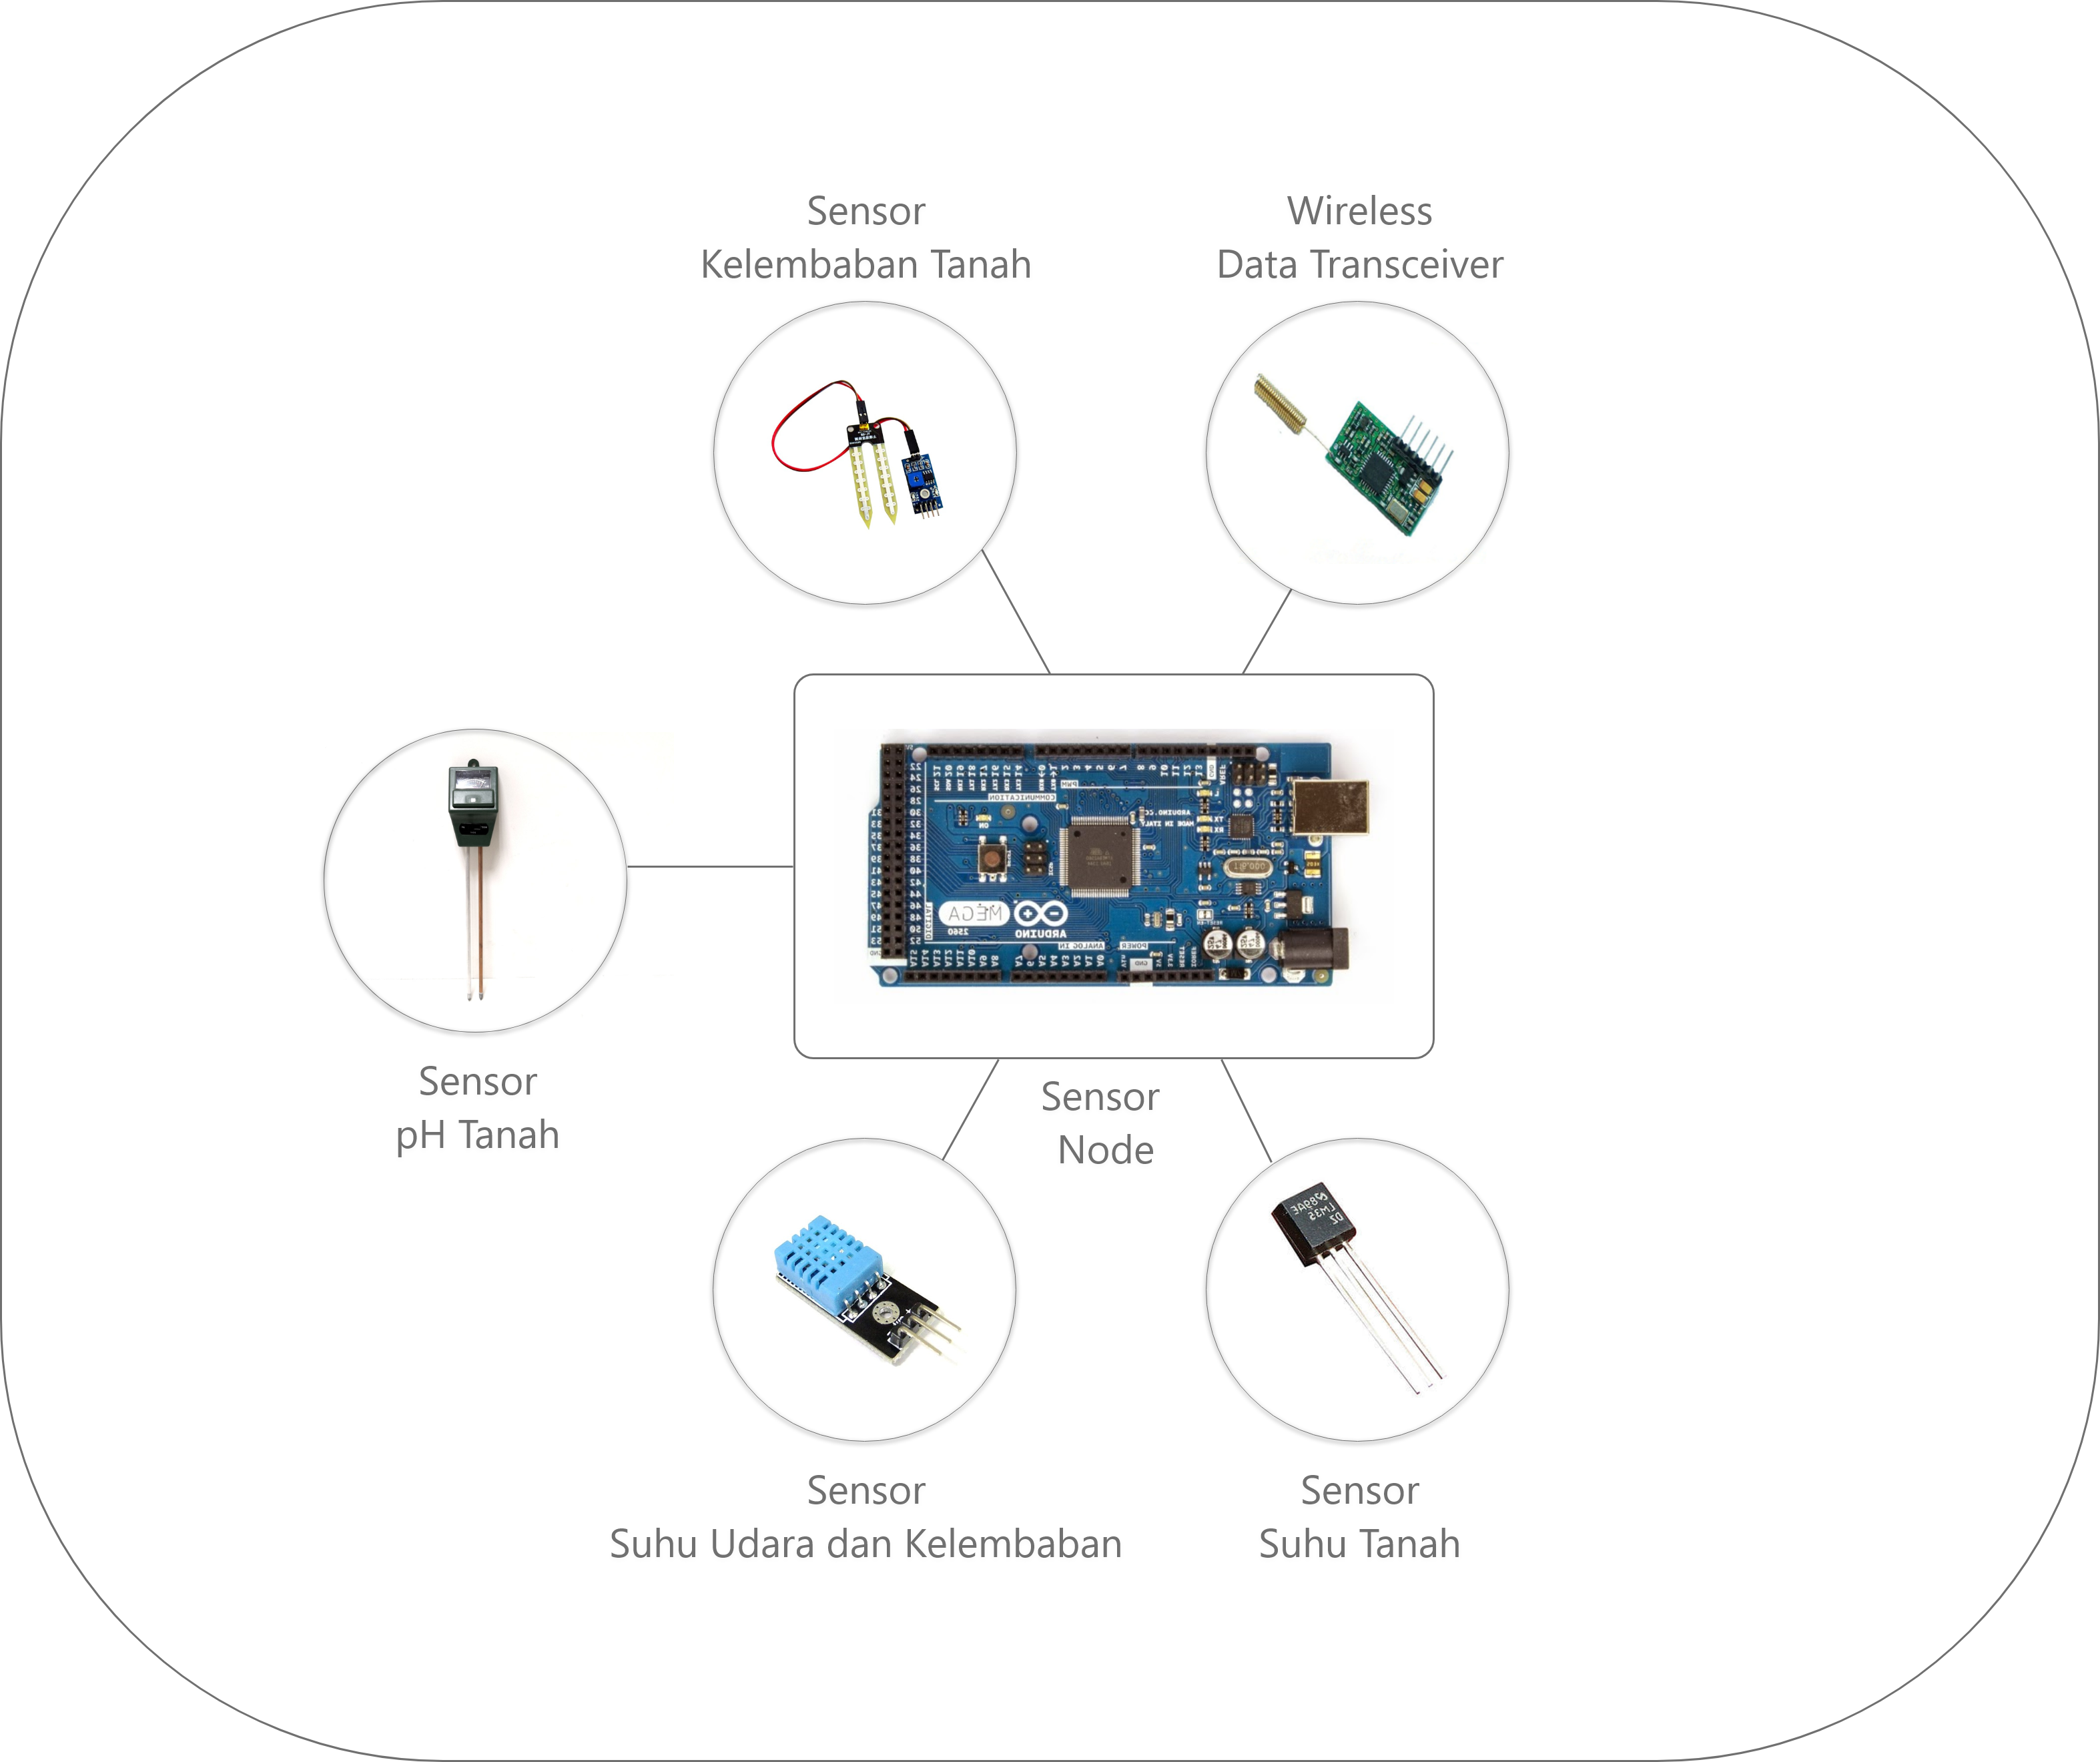
\includegraphics[scale=0.09]{node_dan_sensor.png}  
    	\caption[Node Sensor]{Node Sensor} 
    	\label{fig:Node Sensor} 
    \end{figure}

    \begin{figure}[H]
    	\centering  
    	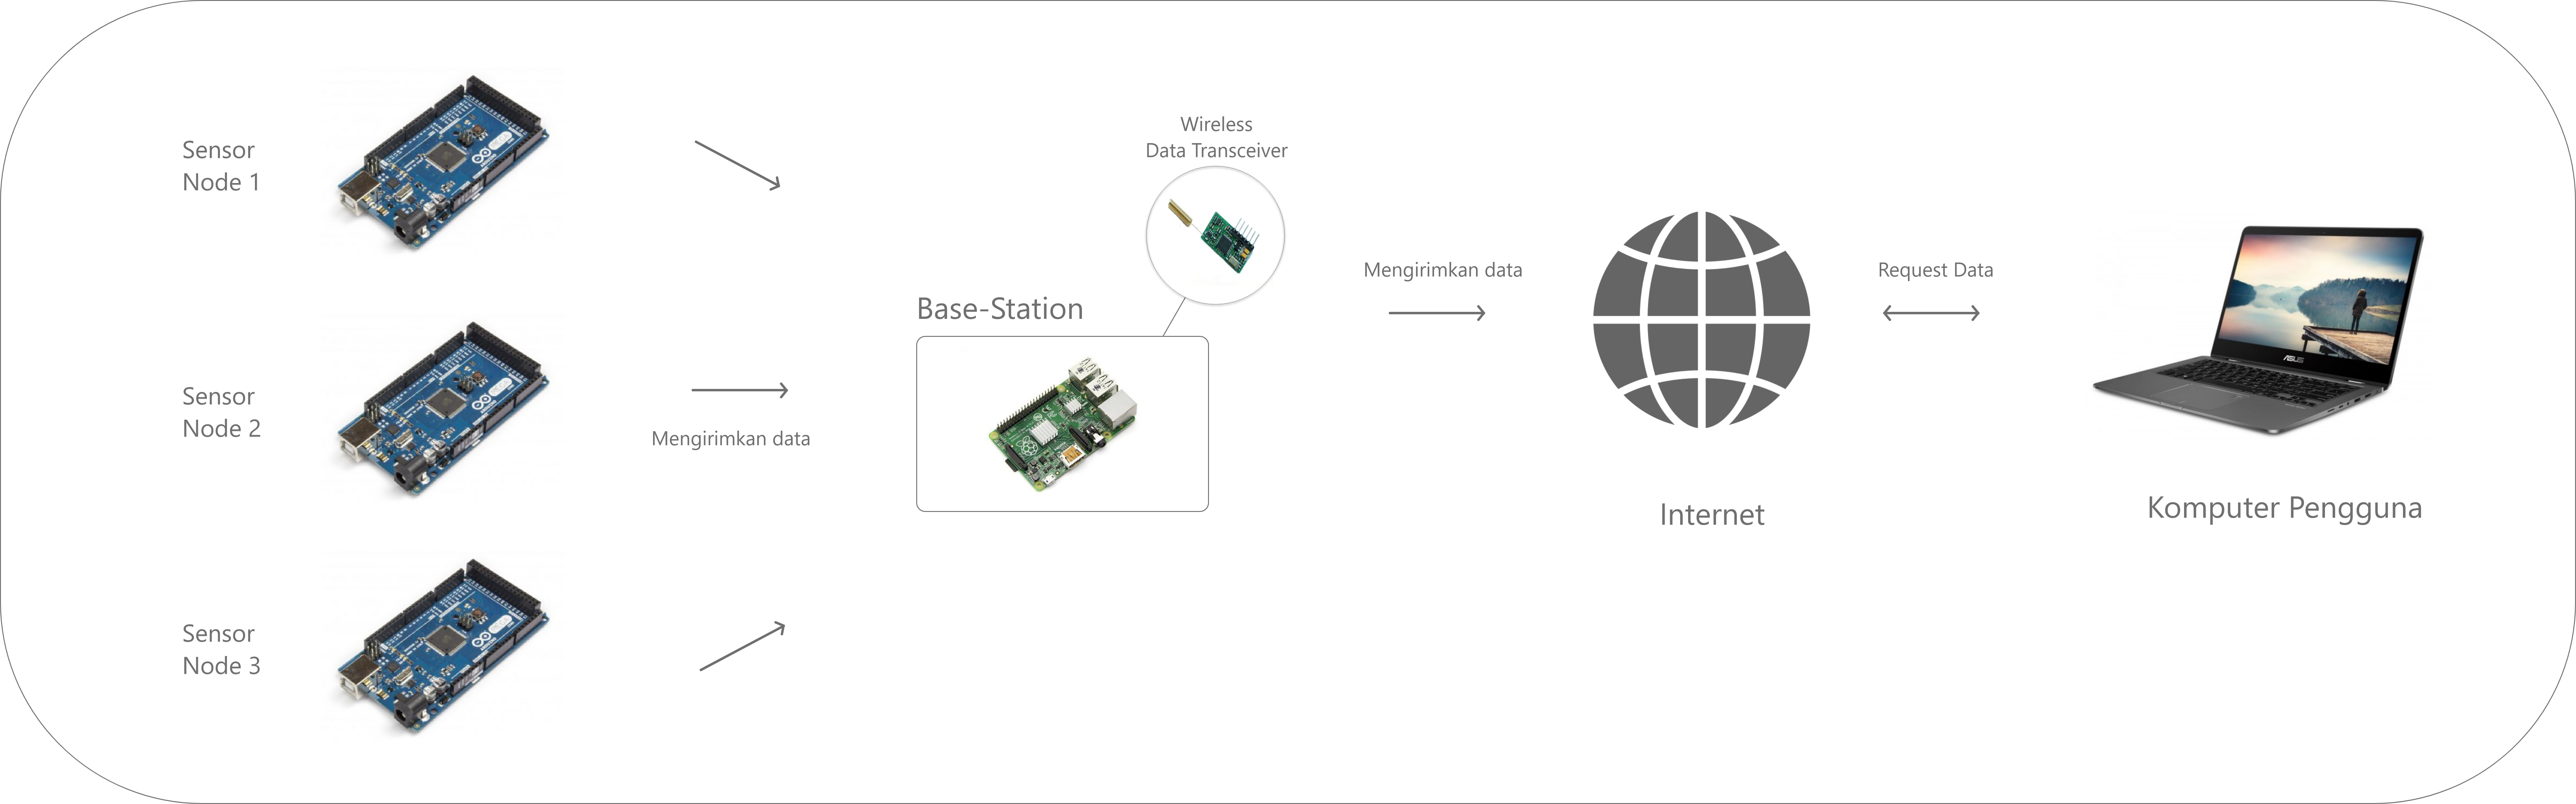
\includegraphics[scale=0.056]{arsitektur_rev.png}  
    	\caption[Arsitektur dan Topologi WSN]{Arsitektur dan Topologi WSN} 
    	\label{fig:Arsitektur dan Topologi WSN} 
    \end{figure}

\section{Analisis Perangkat lunak}
     Perangkat keras yang dibutuhkan dalam melakukan pemantauan kondisi tanah padi terdiri dari node sensor dan sensor \textit{sensing}. Kedua perangkat tersebut akan dirakit sebelum disebar pada area yang diteliti. Masing-masing node sensor memiliki sejumlah sensor \textit{sensing} untuk melakukan pengambilan informasi tanah sawah, seperti kadar keasaaman tanah (pH), kelembaban tanah, dan suhu tanah. Selain sensor \textit{sensing} untuk tanah, node sensor yang disebar juga memiliki sensor \textit{sensing} udara yang dapat mendeteksi suhu dan kelembaban udara persawahan. Modul terakhir yang terpasang pada node sensor adalah \textit{Wireless Data Transceiver} yang berfungsi untuk mengirimkan dan menerima data antar node sensor maupun dengan \textit{base station}.
     
     Setelah perangkat keras telah siap untuk digunakan, proses yang akan dilakukan adalah menyebarkan beberapa node sensor di area persawahan yang diteliti. Letak ataupun bentuk penyebaran node sensor yang dilakukan bergantung pada jenis topologi yang akan diuji. Sensor sensing pada setiap node akan mengambil data tanah sawah yang diteliti dan akan diterima oleh node sensor.
     
     Node sensor akan menyimpan informasi hasil \textit{sensing} yang diterima untuk diteruskan ke \textit{base-station}. Jika jarak suatu node sensor terlalu jauh dengan \textit{base station}, maka data hasil \textit{sensing} akan dikirimkan ke node sensor yang berdekatan dengannya (dan lebih dekat dengan \textit{base station}) untuk meneruskan data hasil \textit{sensing}nya ke \textit{base station}. Node sensor akan saling berkomunikasi dan saling bertukar data sampai data tersebut sampai ke \textit{base station}. Setelah data sampai di \textit{base station}, maka data tersebut akan disimpan dalam database server. Data-data yang tersimpan akan diteruskan oleh \textit{base station} ke komputer untuk ditampilkan pada pengguna dan/atau admin. 


    \begin{figure}[H]
    	\centering  
    	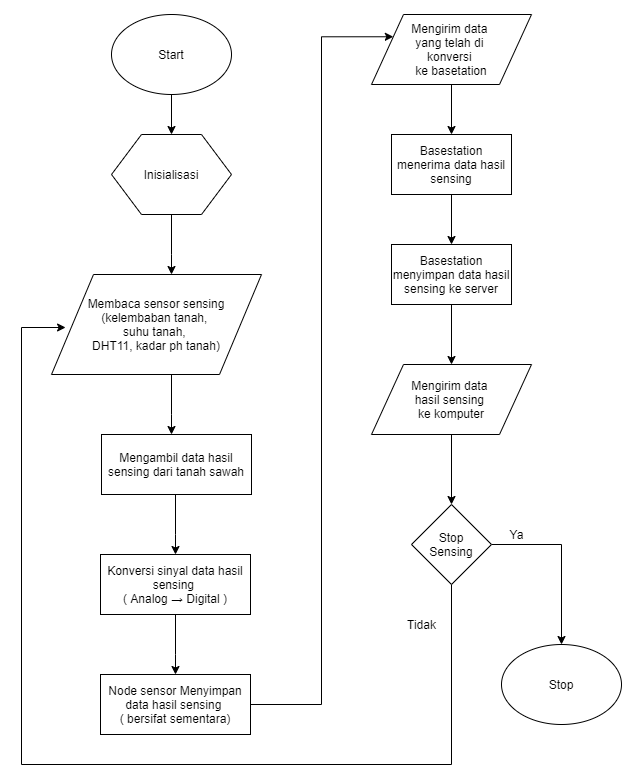
\includegraphics[scale=0.55]{2021_flowchart.png}  
    	\caption[Flowchart keseluruhan sistem]{Flowchart keseluruhan sistem} 
    	\label{fig:Flowchart keseluruhan sistem} 
    \end{figure}

\subsection{Analisis Fungsi Aplikasi} \label{Analisis Fungsi Aplikasi}
Aplikasi yang dibangun memiliki fungsi-fungsi sebagai berikut :
\begin{enumerate}
    \item Memeriksa status pada setiap node sensor
    \item Menyamakan waktu pada setiap node sensor
    \item Mengirimkan perintah untuk melakukan \textit{sensing} pada seluruh node
    \item Mengirimkan perintah untuk menghentikan aktifitas \textit{sensing} pada seluruh node
    \item Mengubah data hasil \textit{sensing} dari sinyal analog menjadi sinyal digital
    \item Menyimpan hasil konversi hasil \textit{sensing} di node sensor
    \item Mengirimkan data hasil \textit{sensing} ke \textit{base station}
    \item Menyimpan data hasil \textit{sensing} yang diterima \textit{base station}
    \item Menampilkan data hasil \textit{sensing} yang disimpan oleh \textit{base station}
\end{enumerate}

Aplikasi memiliki fungsi untuk memeriksa status untuk setiap node sensor yang disebar. Fungsi ini memastikan sensor dalam jaringan yang ada akan melakukan \textit{sensing} berstatus aktif, sebelum melakukan pengiriman data ke \textit{base station}. Jika terdapat sensor yang tidak dalam status aktif, maka aplikasi akan memberi informasi node yang tidak aktif tersebut dan pengguna dapat melakukan perbaikan terlebih dahulu.

Fungsi menyamakan waktu pada setiap node sensor diperlukan agar setiap node mengirimkan data hasil \textit{sensing} secara bersamaan atau pada waktu yang sama. Selain itu \textit{memory} di setiap node sensor yang bersifat sementara (\textit{volatile}), juga menjadi alasan perlunya penyamaan waktu. Karena aplikasi perlu mencatat waktu terakhir setiap node sensor tersebut mati, agar dapat kembali melakukan konfigurasi waktu, dan node dapat kembali melakukan \textit{sensing} secara bersamaan.

Aplikasi yang dibangun juga memiliki fungsi untuk memberikan perintah kepada node sensor yang disebar untuk melakukan \textit{sensing}. Ketika proses pemantauan selesai maka aplikasi juga dapat memberikan perintah untuk menghentikan kegiatan \textit{sensing} pada setiap node sensor.

Fungsi konversi data hasil \textit{sensing} digunakan untuk mengubah sinyal hasil \textit{sensing} yang berupa sinyal analog menjadi sinyal digital. Hasil konversi ini akan langsung dikirimkan ke \textit{base station} dan disimpan di server atau \textit{localhost}. \textit{Base station} akan meneruskan data hasil \textit{sensing} yang diterimanya ke komputer.

Fungsi yang terakhir merupakan fungsi antarmuka. Antarmuka pada aplikasi yang dibangun dapat menampilkan data hasil \textit{sensing} di layar komputer pengguna. Selain itu, antarmuka juga menjadi perantara untuk pengguna, untuk berinteraksi dengan \textit{base station} dan node sensor. 

    \begin{figure}[H]
    	\centering  
    	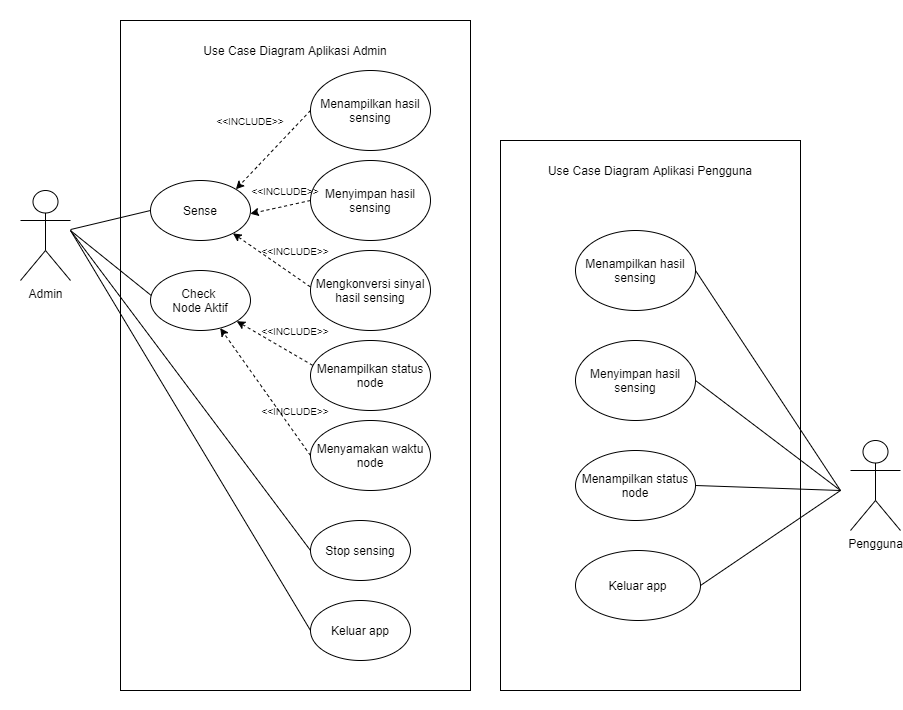
\includegraphics[scale=0.52]{usecase_revisi_final.png}  
    	\caption[Use Case Diagram Aplikasi]{Use Case Diagram Aplikasi} 
    	\label{fig:Use Case Diagram Aplikasi} 
    \end{figure} 
    

    \begin{table}[H]
        \centering
        \caption{Tabel Skenario Memeriksa Status Node Sensor Aplikasi Admin}
        \begin{tabular}{|p{3cm}|p{10cm}|}
        \hline
            Nama & \textit{Check Status Node}\\
        \hline 
        \hline
            Deskripsi & Memeriksa status node sensor agar siap untuk melakukan \textit{sensing}. Base-station akan mengirim sinyal kepada seluruh node yang terhubung dalam jaringan. Jika node aktif, maka node akan mengirim data status node untuk ditampilkan pada aplikasi Admin. Jika sensor tidak aktif maka tidak ada sinyal atau data yang dapat dikirimkan. Aplikasi juga menyamakan waktu pada setiap node sensor dengan komputer pengguna\\
        \hline
            Aktor & Admin\\
        \hline
            Pre-kondisi & Aplikasi Admin sudah dibuka\\
        \hline
            Alur Skenario Utama & 
             \begin{enumerate}
                \item Sistem menampilkan opsi fitur (menu utama) aplikasi admin yang dapat dipilih oleh admin.
                
                \item Admin memilih opsi \textit{"Check Status Node"}
                
                \item Admin menginput opsi untuk mengeksekusi "Check Status Node"
                
                \item Sistem mengirim sinyal ke seluruh Node yang terhubung dalam jaringan untuk mengirim status node
                
                \item Sistem menampilkan dialog "Mengirim perintah check status" dan "Silakan tunggu respon"
                
                \item Sistem menunggu waktu \textit{time-out} dan menerima status node yang dikirimkan oleh node sensor yang aktif dan terhubung dalam jaringan
                
                \item Sistem menampilkan node yang berstatus aktif
                
                \item Sistem menampilkan dialog "Check Node Selesai" bila terdapat node yang merespon perintah 'check status node'
                
                \item Sistem menampilkan dialog "Tidak ada respon" dan "Silakan Check Perangkat", jika tidak ada node yang merespon perintah 'check status node'
                
                \item Sistem kembali menampilkan menu utama aplikasi admin
                
                % \item Aplikasi menampilkan pesan \textit{"Ready to Execute"} jika seluruh node telah dalam status aktif atau \textit{"Online"}
            \end{enumerate}\\
            \hline
        \end{tabular}
        \label{tab:skenario4}
    \end{table}
    
    
    \begin{table}[H]
        \centering
        \caption{Tabel Skenario Perintah \textit{Sensing} Aplikasi Admin}
        \begin{tabular}{|p{3cm}|p{10cm}|}
        \hline
            Nama & \textit{Mulai Sensing}\\
        \hline 
        \hline
            Deskripsi & Memberikan perintah untuk mengeksekusi proses \textit{sensing} pada seluruh node sensor, mengubah sinyal hasil \textit{sensing}, dan melakukan pengiriman data oleh \textit{base station}, serta menampilkannya pada komputer\\
        \hline
            Aktor & Admin \\
        \hline
            Pre-kondisi & Aplikasi sudah aktif dan seluruh status node telah \textit{"online"}\\
        \hline
            Alur Skenario Utama & 
             \begin{enumerate}
                \item Sistem menampilkan opsi fitur (menu utama) aplikasi yang dapat dipilih oleh admin.
                \item Admin memilih opsi \textit{"Mulai Sensing"}
                \item Admin menginput opsi untuk mengeksekusi "Mulai Sensing"
                \item Sistem menampilkan dialog "Sensing dimulai.."
                \item \textit{Base station} mengirimkan perintah sensing pada setiap node yang terhubung dalam jaringan
                \item Node yang terhubung dalam jaringan menerima perintah \textit{sensing} dan melakukan proses \textit{sensing} dan pemantauan
                \item Sistem pada node mengubah sinyal hasil \textit{sensing} dari analog ke digital
                \item Sistem pada node mengirim hasil sensing ke base-station
                \item Aplikasi admin menerima hasil sensing yang dikirimkan oleh node sensor
                \item Aplikasi admin menampilkan hasil sensing yang diterima dan menyimpan hasil \textit{sensing} tersebut
            \end{enumerate}\\
        \hline
        \end{tabular}
        \label{tab:skenario4}
    \end{table}
    
    \begin{table}[H]
        \centering
        \caption{Tabel Skenario Memeriksa Status Node Sensor Aplikasi Pengguna}
        \begin{tabular}{|p{3cm}|p{10cm}|}
        \hline
            Nama & \textit{Check Status}\\
        \hline 
        \hline
            Deskripsi & Memeriksa status node sensor agar siap untuk melakukan \textit{sensing}, jika sensor aktif maka akan menampilkan status \textit{"online"}, sebaliknya jika sensor tidak aktif maka akan ditampilkan status \textit{"offline"}. Aplikasi juga menyamakan waktu pada setiap node sensor dengan komputer pengguna\\
        \hline
            Aktor & Pengguna dan Admin\\
        \hline
            Pre-kondisi & Aplikasi Pengguna sudah dibuka\\
        \hline
            Alur Skenario Utama & 
             \begin{enumerate}
                \item Aplikasi menampilkan opsi fitur aplikasi yang dapat dipilih oleh pengguna.
                
                \item Pengguna memilih opsi \textit{"Check Status Node"}
                
                \item Aplikasi menampilkan halaman check status node
                
                \item Aplikasi menampilkan status node di komputer Pengguna
                
                
            \end{enumerate}\\
            \hline
        \end{tabular}
        \label{tab:skenario4}
    \end{table}
    
    
     \begin{table}[H]
        \centering
        \caption{Tabel Skenario Perintah \textit{Sensing} Aplikasi Pengguna}
        \begin{tabular}{|p{3cm}|p{10cm}|}
        \hline
            Nama & \textit{Mulai Sensing}\\
        \hline 
        \hline
            Deskripsi & Menampilkan data hasil sensing yang tersimpan di basis data. Proses \textit{sensing} pada seluruh node sensor yang yang telah dikirimkan ke base-station akan disimpan di basis data, dan akan ditampilkan pada aplikasi pengguna\\
        \hline
            Aktor & Pengguna dan Admin \\
        \hline
            Pre-kondisi & Aplikasi sudah aktif dan seluruh status node telah \textit{"online"}\\
        \hline
            Alur Skenario Utama & 
             \begin{enumerate}
                \item Aplikasi menampilkan opsi fitur aplikasi yang dapat dipilih oleh pengguna.
                \item Pengguna menekan tombol '\textit{Let's get Started}' pada halaman utama atau menekan link 'Sensing' yang berada di header
                \item Aplikasi menampilkan halaman sensing dan menampilkan tabel data hasil sensing yang didapatkan secara \textit{real-time}
                \item Aplikasi melakukan \textit{refresh} halaman \textit{sensing} secara berkala untuk memperbarui tabel data hasil \textit{sensing}
            \end{enumerate}\\
        \hline
        \end{tabular}
        \label{tab:skenario4}
    \end{table}
    
    \begin{table}[H]
        \centering
        \caption{Tabel Skenario Menghentikan \textit{Sensing} Aplikasi Admin}
        \begin{tabular}{|p{3cm}|p{10cm}|}
        \hline
            Nama & \textit{Stop Sensing}\\
        \hline 
        \hline
            Deskripsi & Memberikan perintah untuk menghentikan proses \textit{sensing} pada seluruh node sensor dan pengiriman data ke \textit{base station}\\
        \hline
            Aktor & Admin \\
        \hline
            Pre-kondisi & \textit{Base station} belum mengirimkan perintah sensing pada node sensor yang terhubung dalam jaringan\\
 
        \hline
            Alur Skenario Utama & 
             \begin{enumerate}
                \item Sistem menampilkan data hasil sensing yang diterima oleh base station
                \item Admin memilih opsi "Stop Sensing"                 
                \item Admin menginput opsi untuk mengeksekusi "Stop Sensing" 
                \item Base Station mengirimkan perintah hentikan sensing pada setiap node yang terhubung dalam jaringan
                \item Node yang terhubung dalam jaringan menerima perintah hentikan sensing dan menghentikan seluruh aktifitas sensing
                \item Aplikasi Admin menampilkan dialog "Sensing dihentikan !"
                \item Aplikasi menampilkan kembali menu utama aplikasi Admin
                
            \end{enumerate}\\
        \hline
        \end{tabular}
        \label{tab:skenario4}
    \end{table}
    
    
    
    \begin{table}[H]
        \centering
        \caption{Tabel Skenario Keluar Aplikasi Aplikasi Admin}
        \begin{tabular}{|p{3cm}|p{10cm}|}
        \hline
            Nama & Matikan Aplikasi Base Station\\
        \hline 
        \hline
            Deskripsi & Memberikan perintah untuk menghentikan proses \textit{sensing} pada seluruh node sensor dan pengiriman data oleh \textit{base station}, serta keluar dari aplikasi\\
        \hline
            Aktor & Admin \\
        \hline
            Pre-kondisi & Aplikasi sedang melakukan \textit{sensing} dan \textit{transfer} data, ataupun aplikasi tidak sedang melakukan kegiatan pemantauan \\
        \hline
            Alur Skenario Utama & 
             \begin{enumerate}
                \item Pengguna memilih opsi \textit{"Matikan Aplikasi Base Station"} 
                \item Aplikasi menghentikan segala proses \textit{sensing} dan pemantauan, jika sedang dilakukan.
                \item Aplikasi menampilkan pop-up dialog konfirmasi keluar dari aplikasi
                \item Keluar dari aplikasi
            \end{enumerate}\\
        \hline
        \end{tabular}
        \label{tab:skenario4}
    \end{table}
    
    \begin{table}[H]
        \centering
        \caption{Tabel Skenario Keluar Aplikasi Aplikasi Pengguna}
        \begin{tabular}{|p{3cm}|p{10cm}|}
        \hline
            Nama & Keluar Program\\
        \hline 
        \hline
            Deskripsi & Memberikan perintah untuk menghentikan proses \textit{sensing} pada seluruh node sensor dan pengiriman data oleh \textit{base station}, serta keluar dari aplikasi\\
        \hline
            Aktor & Pengguna dan Admin \\
        \hline
            Pre-kondisi & Aplikasi sedang melakukan \textit{sensing} dan \textit{transfer} data, ataupun aplikasi tidak sedang melakukan kegiatan pemantauan \\
        \hline
            Alur Skenario Utama & 
             \begin{enumerate}
                \item Pengguna memilih opsi \textit{"Keluar Aplikasi"} yang disediakan oleh browser
 
                \item Keluar dari aplikasi
            \end{enumerate}\\
        \hline
        \end{tabular}
        \label{tab:skenario4}
    \end{table}
     
    
\subsection{Analisis Kelas} \label{Analisis Kelas}
Perangkat lunak yang dibangun memiliki pemodelan konseptual umum dari suatu struktur aplikasi, menggunakan kelas diagram. Dengan diagram kelas, objek-objek yang akan dibangun pada perangkat lunak akan lebih mudah untuk dirinci dan diterjemahkan, ataupun dijelaskan. Kelas-kelas yang dirancang ditujukan untuk memudahkan mengetahui fungsi-fungsi yang dimiliki oleh node sensor dan \textit{base station}.

\begin{itemize}
    \item Kelas Diagram Node Sensor

    \begin{figure}[H]
    	\centering  
    	\includegraphics[scale=0.78]{Node_Sensor_fix_lastday.png}
    	\caption[Kelas Diagram Node Sensor]{Kelas Diagram Node Sensor} 
    	\label{fig:Kelas Diagram Node Sensor} 
    \end{figure}
    
    Keterangan
    \begin{itemize}
        \item Kelas Node Sensor
        
        Kelas node sensor mempresentasikan tentang atribut yang dimiliki oleh node sensor dan fungsi-fungsi yang dapat dilakukan oleh node sensor. Node sensor memiliki atribut node untuk memberikan identitas node. 
        
        Method-method yang dimiliki oleh kelas ini antarlain method bacaSensorsSnsing dan method transmisiPengiriman. Method bacaSensorSensing berfungsi untuk mengambil data sensing yang dikirimkan oleh sensor sensing. Method lainnya adalah method statusNode dan statusSensing untuk mengetahui status keaktifan node dan status \textit{sensing} node. Method yang digunakan untuk mengirim data hasil sensing ke \textit{base station} adalah transmisiPengiriman yang memiliki paramater untuk memasukan data yang akan dikirimkan oleh node sensor. 
        
        % \item Kelas Sensor \textit{Sensing} 
        
        % Kelas Sensor \textit{Sensing} memodelkan sensor \textit{sensing} yang terhubung dengan node sensor. Kelas ini memiliki atribut yang mirip dengan kelas node sensor. Namun pada kelas sensorSensing, tipe data dari dataSensing adalah FORMAT.
        % Methods-methods yang terdapat dikelas ini adalah \textit{setter} dan \textit{getter} (\textit{receive}) dari setiap atribut yang berada di kelas SensorSensing
        
        % \item Relasi
        
        % Relasi kedua kelas ini adalah \textit{one-to-many}, sebuah node dapat memiliki lebih dari satu (minimal nol) sensor \textit{sensing}, dan sebuah sensor minimal terhubung ke sebuah node.
    \end{itemize}
    
    
    \item Kelas Diagram \textit{Base station}
    
    \begin{figure}[H]
    	\centering  
    	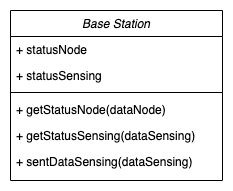
\includegraphics[scale=0.78]{BS_Class_fixing_lastday.png}
    	\caption[Kelas Diagram \textit{Base station}]{Kelas Diagram \textit{Base station}} 
    	\label{fig:Kelas Diagram Base Station} 
    \end{figure}
    
     
    Keterangan
    \begin{itemize}
        \item Kelas \textit{Base station}
        
        Kelas base stasion memiliki lima atribut dan lima methods. Atribut yang terdapat dikelas ini adalah atribut statusNode dan statusSensing, yang berperan untuk menampung value dari status node dan status sensing yang dikirimkan oleh node sensor.
        
        Kelas ini memiliki method getDataSensing dan method sentDataSensing. Method getDataSensing berperan untuk menerima data yang dikirimkan oleh node sensor. Method sendDataSensing digunakan untuk mengirimkan data hasil \textit{sensing} yang dikirim oleh node sensor dan telah diterima oleh \textit{base station}, ke \textit{server} untuk ditampilkan ke komputer pengguna.
    \end{itemize}
\end{itemize}

\clearpage

\subsection{Analisis Basis Data}

    Basis data yang dirancang, ditujukan untuk menyimpan data hasil sensing di komputer pengguna. 

\begin{itemize}

    \begin{figure}[H]
    	\centering  
    	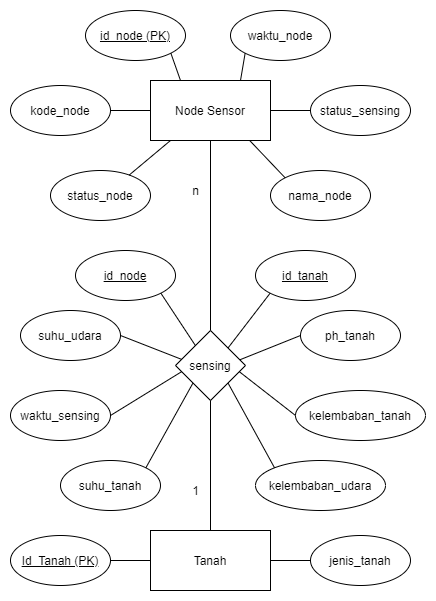
\includegraphics[scale=0.48]{Fixing_ERD_LastDay_Rapih.png}   
    	\caption[ERD Perangkat lunak]{ERD Perangkat lunak} 
    	\label{fig:ERD Perangkat lunak} 
    \end{figure}
    
    \item Rancangan Konseptual Basis Data
        \begin{itemize}
            \item Entitas
            \begin{itemize}
        %  \item Sensor \textit{Sensing}\\
        %  Memiliki Atribut :
        %  \begin{itemize}
        %      \item id sensor
        %      \item nama sensor
        %      \item type sensor
        %      \item status sensor
        %  \end{itemize}
         
        %  Keterangan :
         
        %  \quad Setiap sensor \textit{sensing} memiliki id sensor yang berbeda-beda sesuai dengan node sensor yang terhubung. Sebuah sensor \textit{sensing} memungkinkan untuk memiliki type sensor yang sama dengan sensor \textit{sensing} lainnya. Namun untuk nama sensor, diberi label atau nama berdasarkan type dan node sensor yang terhubung. Atribut status sensor, menunjukan kesiapan sensor untuk melakukan pengambilan data.\\
     \end{itemize}
    
     
    \begin{itemize}
         \item Node Sensor\\
         Memiliki Atribut :
         \begin{itemize}
             \item id node
             \item kode node
             \item nama node
             \item status node
             \item status sensing
             \item waktu node
         \end{itemize}
         
         Keterangan :
         
         \quad Setiap node sensor memiliki id sensor yang berbeda-beda sesuai dengan urutan terhubungnya node sensor dengan \textit{base station}. Atribut kode node dan nama node pada node sensor, didapatkan berdasarkan atribut nama yang dikirimkan oleh node sensor. Atribut status node dan status sensing, menunjukan kesiapan sensor untuk melakukan penerimaan data hasil \textit{sensing} dan pengiriman data. Atribut waktu node menunjukan waktu node dalam melakukan \textit{sensing}.\\
     \end{itemize}
     
  
     \begin{itemize}
         \item Tanah\\
         Memiliki Atribut :
         \begin{itemize}
             \item id tanah
             \item jenis tanah
         \end{itemize}
         
         Keterangan :
         
         \quad Entitas memiliki atribut id tanah yang merupakan kode petak sawah yang dilakukan penelitan. Atribut jenis tanah menunjukan cara pengelolaan air pada tanah sawah yang diteliti.
     \end{itemize}
            
            \item Relasi
            \begin{itemize}

                 
                 \item Node Sensor -- Tanah\\
                 Relasi : \textit{One to Many}\\
                 Keterangan :
                 
                 
                 \quad Sebuah node sensor hanya dapat melakukan \textit{sensing} pada sebuah petak tanah sawah. Namun sebuah petak tanah sawah dapat dilakukan penelitan atau pemantauan oleh lebih dari satu node sensor.\\
                 
            \end{itemize}
            
            \item Tabel Relasi
            \begin{itemize}
                 
                 \item Sensing\\
                 Keterangan :
                  Memiliki Atribut :
                 \begin{itemize}
                     \item id tanah
                     \item id node
                     \item ph tanah
                     \item suhu tanah
                     \item kelembaban tanah
                     \item suhu udara
                     \item kelembaban udara
                 \end{itemize}
                 
                 
                 \quad  Atribut id tanah dan id node berperan untuk menghubungkan entitas node sensor dengan entitas tanah. Atribut pH tanah, suhu tanah, kelembaban tanah, suhu udara, dan kelembaban udara, merupakan informasi yang dimiliki oleh tanah sawah yang digunakan untuk menentukan kualitas tanah sawah. \\
                 
            \end{itemize}
        \end{itemize}
\end{itemize}

\subsection{Analisis Paket/Pesan}
 Pertama-tama admin akan menkonfigurasi node tetangga terdekat dari setiap node, agar paket dapat dikirimkan antar node jika jarak suatu node terlalu jauh untuk dikirimkan ke \textit{base station}. Setelah itu, admin mengonfigurasi waktu pada setiap node, agar proses pengiriman data dilakukan secara bersamaan. Ketika kedua tahap tersebut telah dilakukan, saat node sensor pertama kali diaktifkan , maka node sensor akan mengganti statusnya dari \textit{offline} menjadi \textit{online}, lalu akan diketahui tujuan data hasil \textit{sensing} yang akan dikirimkan, dan seluruh node memiliki waktu yang sama.
 
 Seluruh node menunggu perintah \textit{sensing} dari komputer pengguna. Ketika pengguna memberikan perintah \textit{sensing}, maka seluruh node sensor akan melakukan pengambilan data. Data-data yang diambil dari tanah yang diuji, akan dikonversi menjadi sinyal digital dan dikirimkan menuju \textit{base station}. \textit{base station} akan menerima data hasil \textit{sensing} secara terus menerus dan menyimpannya ke server, untuk ditampilkan di komputer pengguna.